\documentclass{tudelft-report}
\usepackage{acronym}
\usepackage{lscape}
\usepackage{gensymb}
\usepackage{textcomp}
\usepackage{multicol}
\usepackage[version=3]{mhchem} % Package for chemical equation typesetting
\usepackage{siunitx} % Provides the \SI{}{} and \si{} command for typesetting SI units
\usepackage{graphicx} % Required for the inclusion of images
\usepackage{natbib} % Required to change bibliography style to APA
\usepackage{amsmath} % Required for some math elements 
\usepackage{hyperref}


\begin{document}

%% Use Roman numerals for the page numbers of the title pages and table of
%% contents.
\frontmatter

\title[Detection of Featureless Objects]{Efficient Gate Detection for Autonomous Drone Racing}
\author{P.\ Duernay}
\affiliation{Delft University of Technology}
%\coverimage{cover.jpg}
%\makecover

%% Include an optional title page.
\begin{titlepage}
	
	\begin{center}
		
		%% Insert the TU Delft logo at the bottom of the page.
		\begin{tikzpicture}[remember picture,overlay]
		\node at (current page.south)[anchor=south,inner sep=0pt]{
			
\includegraphics{cover/logo}
		};
		\end{tikzpicture}
		
		%% Extra whitespace at the top.
		\vspace*{2\bigskipamount}
		
		%% Print the title in cyan.
		{\makeatletter
			\titlestyle\color{tudelft-cyan}\Huge\@title
			\makeatother}
		
		%% Print the optional subtitle in black.
		{\makeatletter
			\ifx\@subtitle\undefined\else
			\bigskip
			\titlefont\titleshape\LARGE\@subtitle
			\fi
			\makeatother}
		
		\bigskip
		\bigskip
		
		by
		%door
		
		\bigskip
		\bigskip
		
		%% Print the name of the author.
		{\makeatletter
			\titlefont\Large\bfseries\@author
			\makeatother}
		
		\vfill
		
		in partial fulfillment of the requirements for the degree of
		%in overeenstemming met de vereisten voor het verkrijgen van de graad van
		
		\bigskip
		\bigskip
		
		{\bfseries Master of Science}
		
		in Embedded Systems
		
		\bigskip
		\bigskip
		
		at the Delft University of Technology,
		%aan de Technische Universiteit Delft,
		
		to be defended publicly on Tuesday January 1, 2013 at 10:00 AM.
		%in het openbaar de verdedigen op dinsdag 1 januari om 10:00 uur.
		
		\vfill
		
		\begin{tabular}{lll}
			%% Add additional information here, per faculty requirements, e.g
			%    Student number: & 1234567 \\
			%    Project duration: & \multicolumn{2}{l}{March 1, 2012 -- January 1, 2013} \\
			Supervisor: & Prof.\ dr.\ ir.\ D. M. J\ Tax \\
			Thesis committee:
			& Prof.\ dr.\ C.\ F.\ Guido de Croon, & TU Delft \\
			& Dr.\ E.\ L.\ Brown, & TU Delft \\
			& Ir.\ M.\ Scott, & Acme Corporation
		\end{tabular}
		
		%% Only include the following lines if confidentiality is applicable.
		\bigskip
		\bigskip
		\emph{This thesis is confidential and cannot be made public until December 31, 2013.}
		%\emph{Op dit verslag is geheimhouding van toepassing tot en met 31 december 2013.}
		
		\bigskip
		\bigskip
		An electronic version of this thesis is available at \url{http://repository.tudelft.nl/}.
		%Een elektronische versie van dit verslag is beschikbaar op \url{http://repository.tudelft.nl/}.
		
	\end{center}
	
\end{titlepage}



\chapter*{Preface}
\setheader{Preface}

Preface\ldots


\begin{flushright}
	{\makeatletter\itshape
		\@author \\
		Delft, January 2013
		\makeatother}
\end{flushright}



\tableofcontents

%% Use Arabic numerals for the page numbers of the chapters.
\mainmatter

\chapter*{Summary}
\addcontentsline{toc}{chapter}{Summary}
\setheader{Summary}

\ac{MAV} are an emerging technology that supports a wide range of applications. Thereby the robust estimation of an \ac{MAV}'s state within its environment is crucial to ensure safe operation. In  indoor scenarios cameras are one of the predominant choices for state estimation sensors. This requires Computer Vision algorithms to interpret the obtained high dimensional signal. An application that allows the competitive evaluation of control and state estimation algorithms is \ac{MAV} Racing such as the \ac{IROS}2018 Autonomous Drone Race. Thereby a race court consisting of several race gates has to be followed. For a fast flight during such a race court the detection of the racing gates with a camera can be used in a high level control loop. As these object consist only of small structures that are spread across large parts of the image, this gives rise to a challenging Object Detection problem.

In recent years \acp{CNN} showed promising results on various vision tasks. However, due to their computational complexity the deployment on mobile devices remains a challenge. Furthermore, \acp{CNN} typically require a vast amount of training data. This work defines the class of \acp{EWFO} and studies their detection on \acp{MAV} with \ac{Yolo}V3. For the training, data is generated with a graphical engine. 

The experiments conducted in simulation show how \acp{EWFO} are harder to detect than filled objects as the detector can be confused to patterns present in the empty part. Particularly for larger objects the detection performance decreases. We give several recommendations how to generate data for the detection of \acp{EWFO} on \acp{MAV}. These include how to include variations in background as well as the camera placement. Finally, we study the incorporation of image augmentation techniques to transfer the detector to the real world. We can report that especially modelling lens distortion improves the performance on the real data. Nevertheless, a reality gap remains that can not fully be explained.

Furthermore, different architectures are studied for the detection of \acp{EWFO}. It can be seen how a relatively shallow network of 9 layers can be used for the detection of \acp{EWFO} on \acp{MAV}. A further reduction in weights leads to a gradual decrease in performance. 

Based on the gained insights the deployment of a detector on an example system is studied. A detection performance/speed trade-off is evaluated. The final detector achieves 32\% $ap_{60}$ at a frame rate of 12 Hz on a real world test set created during this work.



\chapter*{Glossary}
\begin{acronym}
	\acro{IR}{Infrared}
	\acro{LIDAR}{Light Detection And Ranging}
	\acro{EWFO}{Empty Wire Frame Objects}
	\acro{FoV}{Field of View}
	\acro{CNN}{Convolutional Neural Network}
	\acro{GPS}{Global Positioning System}
	\acro{GPU}{Graphical Processing Unit}
	\acro{MAV}{Micro-Air Vehicle}
	\acro{DR}{Domain Randomization}
	\acro{TO}{Target Object}
	\acro{DSC}{Depthwise Separable Convolution}
	\acro{IMU}{Inertial Measurement Unit}
	\acrodefplural{IMU}[IMUs]{Inertial Measurement Units}
	\acro{FPV}{First Person View}
	\acro{IROS}{International Conference of Intelligent Robots}
	\acro{i.i.d.}{independently identically distributed}
\end{acronym}
\chapter{Introduction}
\label{sec:intro}
\acresetall
\acp{MAV} such as a Quadrotor-\ac{MAV} displayed in \autoref{fig:mav} are an emerging technology that supports society in a wide range of consumer, industrial and safety applications. For example \acp{MAV} are used to deliver medicine \cite{Shankland2018}, fight fires \cite{KateBaggaley2017} or even find survivors in disaster situations \cite{JoshuaBateman2017}.

\begin{figure}[b]
	\centering
	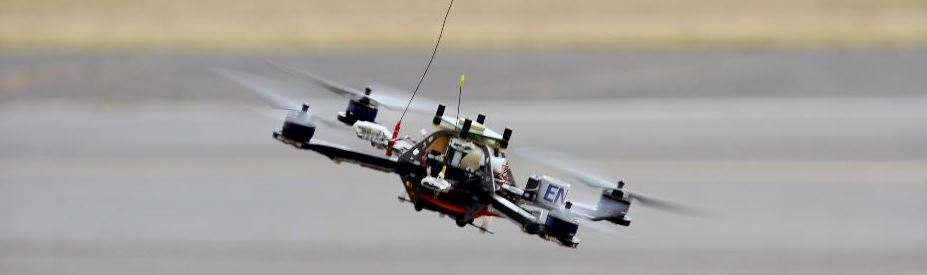
\includegraphics[width=\textwidth]{fig/mav}
	\caption{An example of a Quadrotor-\ac{MAV}-Platform that is used in this thesis.}
	\label{fig:mav}
\end{figure}

Especially in emergency scenarios the fast and safe flight of \acp{MAV} is crucial to deliver help quickly and save human lives. However, due to the complexity of such missions as well as the difficulty to control an \ac{MAV} in disaster scenarios, often multiple human operators are required in order to ensure safe operation \cite{Murphy2016}. With humans in the loop a constant connection between the \ac{MAV} and the operators is required which not only uses energy and requires infrastructure but also significantly increases the reaction time. Enabling \acp{MAV} to fly more autonomously could allow human operators to control more \acp{MAV} and thus to improve the support in emergency situations.

A major challenge on the way to the full autonomous flight of \acp{MAV} is the accurate estimation of the \ac{MAV}'s state within its environment. The system is highly dynamic so position and orientation can change rapidly. At the same time noise introduced by motor vibrations makes the position estimation with only on-board \acp{IMU} too inaccurate \cite{Mohamed2014}. \ac{LIDAR}-sensors can capture long and wide range 3D information but the sensors are typically heavy and require a significant amount of energy. \ac{IR} sensors can cover distance information but are often limited in their \ac{FoV} as well as in their range. External infrastructure like \ac{GPS} and optical tracking systems can provide accurate measurements but there is no guarantee that such systems are present in real world applications. Cameras on the other hand are cheap, lightweight and can measure long range distance information. This makes them a suitable choice as a sensor for on-board state estimation on light \acp{MAV} \cite{Elbanhawi2017}.

However, the signal delivered by the camera is high dimensional and can not directly be interpreted as position or orientation measurements. Computer Vision algorithms are required to interpret the image and extract relevant information. This can be done by designing an algorithm manually or learning the image processing from annotated examples. In particular Deep Learning based methods aim to combine whole Computer Vision pipelines into one mapping that transforms the raw input image into a task dependent output. Experiments have shown how Deep Learning based methods outperform traditional Machine Learning approaches and manually crafted algorithms \cite{Razavian}. This made them the predominant choice for almost any vision task.

The hereby used \acp{CNN} are designed in a hierarchical way, using multiple layers that are evaluated sequentially. An example architecture is displayed in \Cref{fig:cnn_example}. The network transforms an image of size 224x224 from its input (left) to a task dependent output (right). In this case a classification network predicting 1000 class probabilities is displayed. Each layer applies a non-linear transformation for which the parameters are learned during training. By stacking more layers on top of each other (deepening) and increasing the number of nodes $D$ per layer (widening), highly non-linear functions can be modelled. 

Experiments have shown the superior performance of particularly deep/wide models \cite{He, He2015, Szegedy2014, Zagoruyko2016}. However, this model flexibility assumed to be the reason for their superior performance also leads to immense requirements in computational resources. For example a state-of-the-art Computer Vision model \cite{He2015} contains 60.2 million parameters and one inference requires 11.3 billion floating point operations \cite{Tschannen2017}. 

\begin{figure}[bhtp]
	\centering
	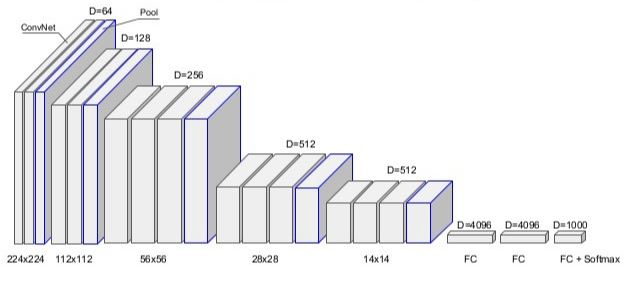
\includegraphics[width=0.8\textwidth]{fig/vgg_architecture}
	\caption{Example Architecture of a \ac{CNN}.}
	\label{fig:cnn_example}
\end{figure}

Robotic platforms like \acp{MAV} have limited resources in terms of processing power and battery life. Hence, the use of \acp{CNN} on such devices is still an open challenge. Research has addressed to reduce the number of computations in Deep Learning models on multiple levels\cite{YoungwanLee, Zagoruyko2016, Howard2017, Ghosh2017, Sandler2018, Zhang2017a}. However, the investigation of relatively shallow models with less than ten layers received only little attention by the research community.

This work investigates the deployment of a Deep Learning based Computer Vision pipeline on a \ac{MAV}. The method is applied in the challenging scenario of Autonomous Drone Racing at the \ac{IROS} 2018. Within the race court several metal gates are placed and need to be passed one after another. Detecting the gates allows to estimate the \ac{MAV}'s relative position and to calculate the flying trajectory. An overview of the race court and the racing gates at the \ac{IROS} 2016 Autonomous Drone Race can be seen in \Cref{fig:race_court}.

\begin{figure}[bhtp]
	\centering
	\begin{minipage}{0.45\linewidth}
	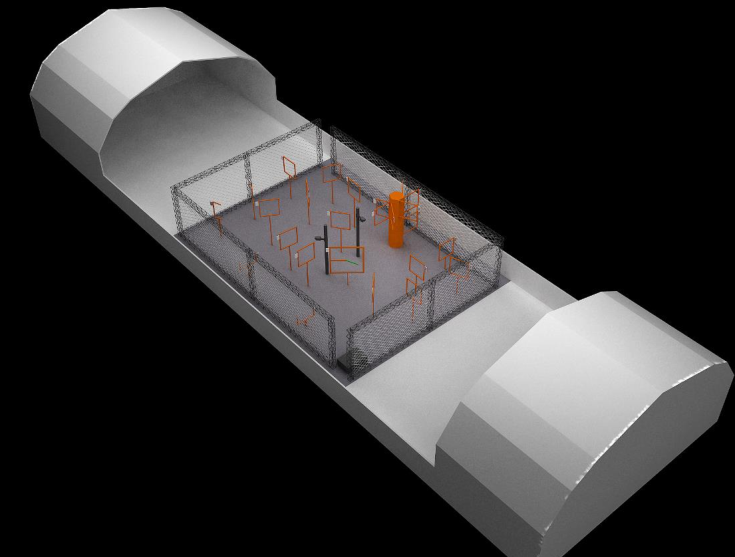
\includegraphics[width=\textwidth]{fig/race_court}
	\end{minipage}\hfill
\begin{minipage}{0.45\linewidth}
	\includegraphics[width=\textwidth]{fig/race_court_side}
\end{minipage}
\caption{Example Images of the \ac{IROS} 2016 Autonomous Drone Race}
\label{fig:race_court}
\end{figure}

The thesis builds on previous work by Ozo et. al \todoref{Reference to Current Method once it is published} which uses a manually crafted image processing method to detect the racing gates. Although fast to execute the method is very sensitive to illumination changes. Moreover, the algorithm fails when the objects are too far away or the frame is very thin. In order to develop a more robust method, this thesis investigates a learning based approach to the detection of racing gates.

Object Detection is one of the most intensively studied topics in Computer Vision. However, the objects investigated are usually solid and contain complex shapes. For example a pedestrian consist of body parts and a face. A box that surrounds the object mostly contains parts with distinctive shape an/or texture. A Computer Vision model can use these features for detection. The racing gates in contrast are of different nature. As can be seen in \Cref{fig:race_court} a box that surrounds the object would largely contain background. Hence, this part can not be used as a hint whether an object is present. Instead it can contain other objects even other gates that might distract a detector. Additionally, the object parts themselves are of very thin structure and can be hardly visible. Thus, a detector needs to make use of fine-grain structures, while ignoring the majority of the image. This introduces a particular vision task that even humans have a hard time at solving \footnote{The unconvinced reader can try to count the number of gates visible in the right image of \Cref{fig:race_court}} and that affects the training and design of a Computer Vision pipeline that aims to detect these kind of objects.

This thesis defines a class of objects as \textbf{\ac{EWFO}} studies methods for their detection. The definition is given as follows:

\paragraph{Definition - Empty Wire Frame Objects}	
\begin{enumerate}
	\item \textbf{Empty.} The object parts are sparse. The bounding box around the object is largely occupied by background.
	\item \textbf{Wire.} The object parts themselves are thin structures. The object does not consist of complex but only basic geometric shapes like corners, lines and edges.
	\item \textbf{Frame.} The object parts can be spread over large parts of the image, while the point of interest is in the center of this part.

\end{enumerate}

The detection of \ac{EWFO} is studied in the examples of the \ac{IROS} drone race gates. These can be seen can be seen in \Cref{fig:gates}. The image shows the \textit{Closed Gate} as well as the \textit{Jungle Gate}. Thereby the orange part is considered to be the object of interest. To the best of the authors knowledge \ac{EWFO} have not been particularly addressed in Computer Vision. In \cite{Falanga} and \cite{Li2018a} the authors also detect racing gates, however the used objects contain more structure than the ones investigated in this thesis. \citeauthor{Jung2018} present a framework to detect similar objects in \cite{Jung} and \cite{Jung2018} but do not study the particular effects of the object shape. This work particularly addresses the implications of the object shape in using a Deep Learning based detection system for \ac{EWFO}.

\begin{figure}[bhtp]
	\centering
	\begin{minipage}{0.45\linewidth}
		\centering
		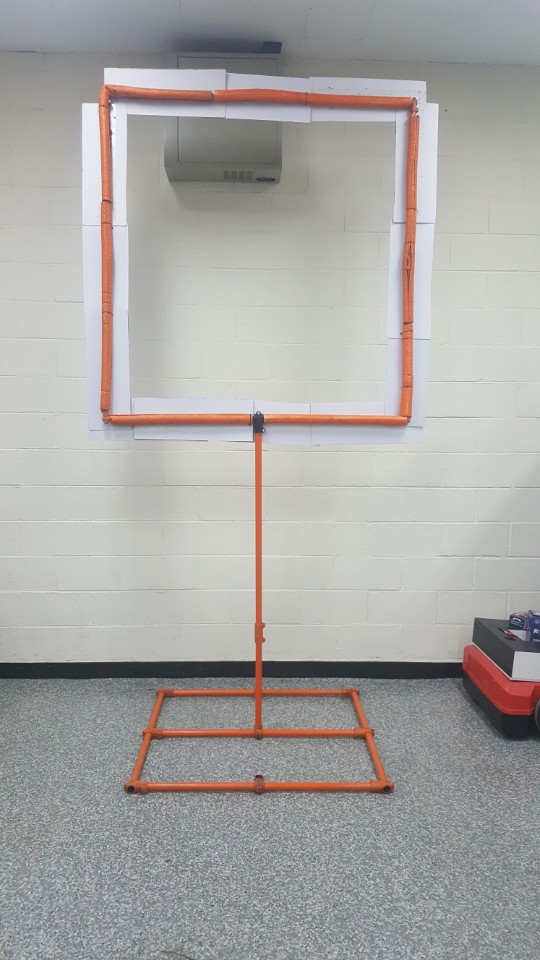
\includegraphics[height=5cm]{fig/closed_real}
	\end{minipage}\hfill
	\begin{minipage}{0.45\linewidth}
		\centering
		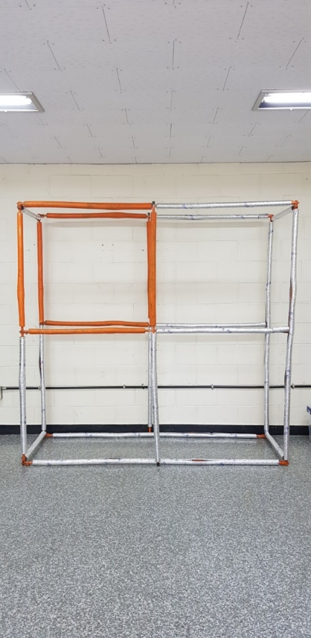
\includegraphics[height=5cm]{fig/jungle_real}
	\end{minipage}
	\caption{Example Images of the Empty Wire Frame Objects investigated in this thesis. }
	\label{fig:gates}
\end{figure}

A drawback of Deep Learning based vision systems is their need for vast amounts of annotated examples, which is not always available. Racing gates for example are not an object that appears often in everyday life and therefore not many example images exist. To this end no publicly available dataset can be used to train a Computer Vision system for \ac{EWFO}. Since a large part of the object consists of background, it is particularly crucial that the training set covers a large variety of backgrounds. Otherwise, it is likely that a model uses the background for prediction and only works in a particular domain (Overfitting). 

\begin{figure}[bhtp]
	\begin{minipage}{0.49\textwidth}
		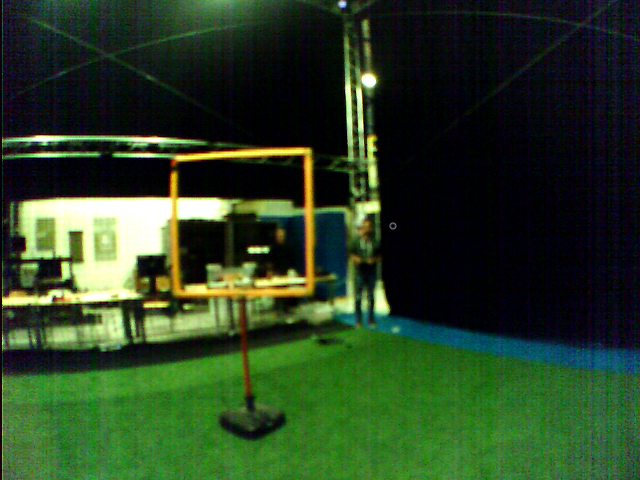
\includegraphics[width=\textwidth]{fig/real_cyberzoo2}
	\end{minipage}
	\begin{minipage}{0.49\textwidth}
		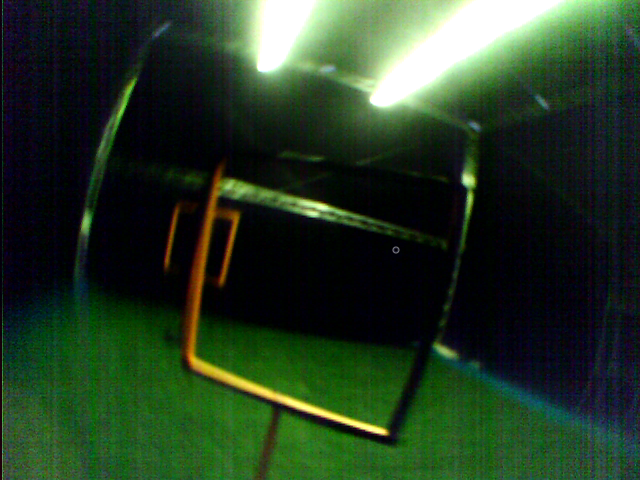
\includegraphics[width=\textwidth]{fig/real_cyberzoo1}
	\end{minipage}
	\label{fig:examples}
	\caption{Example of the \text{Cyberzoo} dataset. On the left an image while the \ac{MAV} is hovering, on the right an image during a turn manoevre.}
\end{figure}

In \Cref{fig:examples} example images of the target domain of this work are displayed. The images are taken during a test flight at a test environment. The left image shows an example when the \ac{MAV} is hovering and thus is in a very stable position. The object in this case is clearly visible as a single orange square. In contrast the right image shows a close up example during a turn manoeuvre. Here it can be seen how the used wide angle lens causes distortion and thus the lines appear as circular shape. Furthermore, large parts of the image including the horizontal bars of the object in the back appear blurred due to the circular velocity of the \ac{MAV}. In addition, the light conditions of the environment significantly influence the object appearance.

While it is possible to remove lens and sensor effects in post-processing, this can lead to information loss and requires on-board resources. Instead it is computationally more efficient to perform the detection on the raw image data. However, sensor effects have been shown to significantly influence the performance of neural networks \cite{Andreopoulos2012,Dodge2016a}. Furthermore, they can lead to varying object appearance on different \acp{MAV}. This further complicates the collection of annotated examples.
 
Another option is the artificial generation of data. By synthetically generating samples with corresponding labels, the theoretical amount of training data is infinite. Moreover, the generation allows to incorporate domain specific properties such as motion blur or image distortion. Hence, data generation is particularly useful for the detection of \acp{MAV} on \acp{EWFO} where a large variety of backgrounds is required while samples are difficult to obtain. Finally, as \ac{MAV} are brittle vehicles and mistakes in development can lead to damage on hardware, engineers and researchers often use simulators to evaluate their systems before transferring them to the real work. Thus the basic infrastructure required to generate data is often already available. 

Yet introduces the generation of data its own challenges. First and foremost because the generation process in itself is based on model assumptions. If these do not sufficiently capture the real world, a model trained in such an environment might be heavily biased and perform poorly in the real world. Secondly, because the generation of visual data is computationally intense. Despite advances in Computer Graphics can virtual environments not yet fully capture the real world. Hence, this work investigates the use of data generation in order to detect \acp{EWFO} on \acp{MAV}.

Without an accurate detection of the racing gate, the \ac{MAV} is not able to determine its current position and thus to calculate its flying trajectory. On the other hand, with an algorithm that requires less computational resources a lighter \ac{MAV} can be built. This allows faster and more aggressive trajectories as well as longer battery life. Moreover, the vision system is part of a greater state estimation and control system which also includes further sensor measurements. Depending on the remaining part of the system, faster and less accurate detections can be more useful than slow but accurate detections. Hence, the trade-off between accuracy and inference speed is of particular interest for this application and is addressed in this work.

\section{Research Question}

This section summarizes the research question addressed in this thesis. Furthermore it describes how the question is split in multiple subquestions that are addressed in the individual chapters.

	\textbf{How can \acp{CNN} detect \ac{EWFO} on \acp{MAV}, using synthetic training data?}


\begin{enumerate}
	\item[\textbf{RQ1}]How can data be generated to train a detection model for \ac{EWFO} detection on a \acp{MAV}?
	\item[\textbf{RQ2}]What kind of architecture is suitable to detect \acp{EWFO}?
	\item[\textbf{RQ3}]What are the trade-offs in detection performance and inference time when a detection model for \acp{EWFO} is deployed on a \ac{MAV}?
	\item[\textbf{RQ4}]Can the gained insights be used to build a lightweight and robust detection model for racing gates in the \ac{IROS} Autonomous Drone Race?
\end{enumerate}

\section{Results/Contributions}

\todo{Put some results at the end.}

\section{Outline}

\todo{Refactor contributions once done}
\begin{figure}[hbtp]
	\centering
	\includegraphics[width=\textwidth]{fig/outline}
	\caption{Thesis Outline}
	\label{fig:outline}
\end{figure}


The thesis is structured as displayed in \Cref{fig:outline}. \Cref{sec:metrics} describes the metrics and systems used for evaluation. \Cref{sec:training}, \Cref{sec:object_detection}, \Cref{sec:tradeoff} and \Cref{sec:method} address the individual research questions. Each chapter contains an introduction to the topic, the methodology used in this thesis and experiments that have been carried out. \Cref{sec:training} describes methods to generate synthetic data for machine learning. It concludes with the datasets used for the remaining parts of this thesis.  \Cref{sec:object_detection} describes object detection and evaluates current methods in the application for \acp{EWFO}. \Cref{sec:tradeoff} illustrates and evaluates measures to reduce computations and optimize an object detection system for a particular hardware. It investigates the trade-off between detection performance and inference time. \Cref{sec:method} describes how the gained insights are used to develop a detector for racing gates at the \ac{IROS} 2018 Autonomous Drone Race. It also compares the current method to a traditional image processing method in terms of speed and detection performance. \Cref{sec:disc} discusses the overall results and formulates a conclusion.




\chapter{Background}
\label{sec:background}
	\section{Object Detection}
	Object Detection is a well studied topic since the very beginning of computer vision. It can be separated in two individual problems which are classification: Which object does the image contain? and localization: Where in the image is the object?.
	
	Existing methods can broadly be grouped in three categories. These are described in the following:

	\subsubsection{Shallow Methods}
	
	Usually filters are handcrafted or learned separately. Their response is fed into a classifier. The detector pipeline is applied on the image in sliding window fashion. The results are filtered by a final non-maximum suppression stage. 
	
	Popular features are haar-features \cite{Viola2004} and the Histogram of Gradients\cite{Forsyth}. These methods give good results as long as the object is fully visible and the position in the test set does not change too much. This issue gave raise to deformable part models where parts of the object are modeled individually and connected with mathematical springs \cite{Viola2004}.
	
	The methods are usually pretty fast but not so accurate.
	
	\subsubsection{Two Stage Detectors}
	
			\paragraph{Scalable Object Detection using Deep Neural Networks\cite{Erhan}}
			\begin{itemize}
				\item[-] Generates number of bounding boxes as object candidates (class agnostic) and confidences for each box
				\item[-] For each Bounding Box a classifier is run e.g. DNN
				\item[-] Training: If the number of boxes k is larger than the number of objects b, only b boxes are matched while the confidence of the others is minimized
				\item[-] Assignment problem $$F_{match}(x,l) = \frac{1}{2}\sum_{i,j}x_{ij}||l_i - g_j||^2_2$$ where $x_ij$ is one if the ith prediction is assigned to the jth ground truth object
				\item[-] Confidence: 
				$$F_{conf}(x,c) = - \sum_{i,j}x_{ij}*\log(c_i)-\sum_{i}(1-\sum_{j}x_{ij})\log{1-c_j}$$
				\item[-] Speed up training by clustering (kmeans) of ground truth and using it as prior (prior matching)
				\item[-] Can be defined to output boxes only for a particular class by training the bounding boxes on that class
				\item[-] Number of parameters grows linearly with number of classes
				\item[-] Authors argue two step process (region proposal + classification) is better
				\item[-] Architecture based on AlexNet
				\item[-] Predicted boxes are merged using non-maxima surpression
				\item[-] One shot(50\%), +2scales (75\%)
				\item[-] OverFeat/ Selective Search are faster but much more expensive
			\end{itemize}
			
	
	Methods consist usually of two stages.An example is R-CNN\cite{Ren}. 
	\begin{itemize}
		\item Object Proposal: A convolutional net proposes regions that contain an object. This is either done in sliding window fashion or in one pass.
		\item Classification: All proposed regions are fed into a classifier. This can either be a "traditional" one or another CNN.
	\end{itemize}
	These methods are usually pretty accurate but also slow.
	\subsubsection{One Stage Detectors}
	
	\begin{figure}[h]
		\centering
		\begin{minipage}{0.4\textwidth}
			\centering
			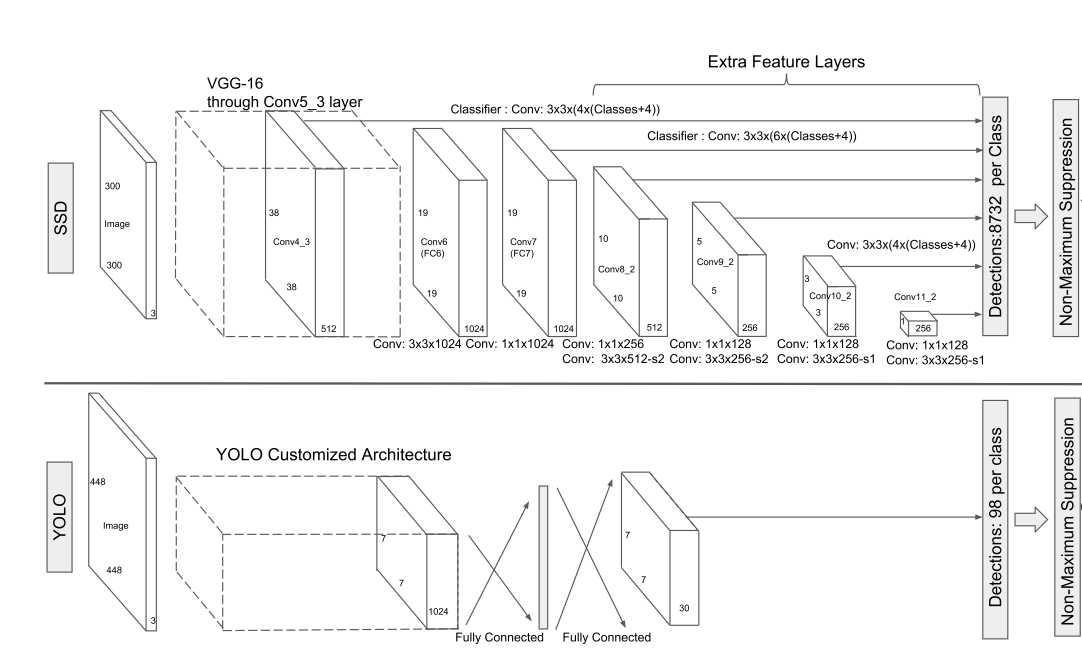
\includegraphics[height=2.5cm]{fig/architecture}
			\caption{Typical Architecture for One Stage Detectors}
			\label{fig:architecture}
		\end{minipage}
		\hspace{2cm}
		\begin{minipage}{0.4\textwidth}
			\centering
			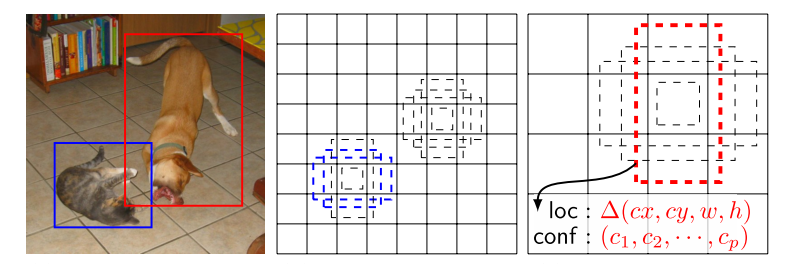
\includegraphics[height=2.5cm]{fig/anchors}
			\caption{Example of \cite{Liu}, the GT box of the cat is matched to two anchor boxes which get responsible for predicting that box. The GT box of the dog is matched to one anchor box.}
			\label{fig:anchors}
		\end{minipage}
	\end{figure}
	
	Most current methods rely on the same principle as Yolo/SSD: A convolutional regression layer is stacked on top of a "base network" that has been trained for image classification e.g. VGG-16. The output layer evaluates feature map(s) of the base network and predicts class confidences, and coordinate offsets for a predetermined set of bounding boxes (so called "prior boxes", "anchor boxes" or "default boxes"). The predictions are filtered in a final non-max-suppression step. During training one has to determine which anchor box is responsible for predicting a certain object. This "matching strategy" differs from method to method but is usually based on the intersection-over-union between the ground truth box and anchor box. \autoref{fig:anchors} illustrates the concept. The final loss function calculates the difference between the responsible boxes and the ground truth. 
	
	Within this framework several approaches exist that either change the base network or modify layers in between: \cite{ChengchengNing2017} propose to include an inception module in the network architecture to reduce computation while keeping/increasing performance. They also propose a more efficient non-max-suppression method. \cite{Wu} uses \textit{SqueezeNet} as base network and a mixture between the ssd and yolo loss function as training goal. \cite{Xiang} investigates the receptive fields of SSD and tries to incorporate more context, especially on lower feature maps, to increase detection rate for small objects.\cite{Linb} applies the framework for vehicle detection. They use \textit{GoogLeNet} as base network (and investigate several others).\cite{TripathiSanDiego} apply a network very similar to YoloV2 and investigate 8bit quantization of the model to make it runnable on embedded devices.
	
	A common problem of one stage detectors is the imbalance between background and object samples. Most methods upweigh the positive samples and/or use hard negative mining. \cite{Lin} introduces the \textit{Focal Loss} which focuses on sparse positive samples by design.
	
	\subsubsection{LCDNet\cite{TripathiSanDiego}}
	
	Aims to bring one shot detection to be runnable on embedded devices.
	
	\begin{itemize}
		\item Quantizies model for inference with 8bit. Records min and max value for each layer and quantizes everything between 0,255
		\item Replaces fully connected layers with convolutional layers
		\item Replaces LeakyRelu with Relu in all but the last (faster?)
		\item Softmax on classification, Sigmoid on confidence
		\item Sigmoid if only one class
		\item quantization mainly effects localization
	\end{itemize}
	
	\subsection{\cite{Linb}}
	
	\begin{itemize}
		\item Uses GoogLeNet as base network
		\item investigates image augmentation and hard negative mining
		\item Uses confidence score plus class probability although only one object shall be detected
	\end{itemize}
		

\begin{table}[]
	
	\caption{Object Detection}
	\label{my-label}
	\begin{tabular}{|p{3cm}|p{3cm}|p{3cm}|p{3cm}|p{3cm}|p{3cm}|p{3cm}|p{3cm}|}
		\hline
		& \multicolumn{3}{l|}{Traditional} & \multicolumn{4}{l|}{Deep}   \\ \hline
		& Viola\&Jones    				   & HoG    & DPM   		   & R-CNN    & YOLO         & SSD & OverFeat \\ \hline
		Feature Detector & Haar					   & HoG    & Multiple Hogs and virtual springs   & Learned by CNN     &  Learned by CNN            & & \\ \hline
		Detection & \multicolumn{3}{l|}{Sliding Window, high filter responses indicate there is an object} & NN in sliding window detects regions for possible objects, For each proposed region a classification is run & Image is split in Grid each Grid spawns Bounding boxes and gives class probabilities & & \\
		\hline
		Accuracy (voc) &  & & & 73.2 mAP & 63.4 mAP & 74.3 mAP & \\ 
		\hline
		Speed & & & & 7 FPS (Faster-RCNN) & 45 FPS & 59 FPS & \\
		\hline
		Strengths & & & & & &  &\\
		\hline
		Weaknesses & & & & & &  &\\
		\hline
		\end{tabular}
		
		\end{table}



\section{Pose Estimation}
\label{sec:pose_estimation}
	\subsection{(Re-) Localization}
	\paragraph{PoseNet: A Convolutional Network for Real-Time 6-DOF Camera Relocalization \cite{Kendall}}
	\begin{itemize}
		\item[-] Relocalizes, is trained on images from the scenes where it is applied	\item[-] Accuracy 2m and 3$\degree$  in 50 km$^2$ outdoors, 0.5m and 5$\degree$ indoors, 5ms per frame
		\item[-] ConvNet 23 layers, Image resolution 224x224
		\item[-] transfer learning from recognition/classification datasets (ConvNet is trained on classification tasks)
		\item[-] based on GoogleNet, affine regressors instead of softmax\item[-] automatic training data generation (structure from motion)
		\item[-] learns p from arbitrary global reference frame
		\item[-] $loss(I) = || \hat{x}-x||_2 + \beta*||\hat{q}-\frac{q}{||q||}||_2$
		\item[-] separating position/orientation led to drop in performance
		\item[-] PoseNet evaluation at single center crop + Dense PoseNet 128 uniformly spaced crops (time increase 95ms, only slight accuracy increase)
		\item[-] Training data generated using structure from motion (Cambridge Scene) and 7 Scenes (Microsoft) for indoor
		
	\end{itemize}
	\paragraph{A Deep Learning Based 6 Degree-of-Freedom
		Localization Method for Endoscopic Capsule Robots \cite{Turan2017}}
	\begin{itemize}
		\item[-] not published yet?
		\item[-] Uses 6-DOF camera pose directly
		\item[-] based on GoogleNet (9 Inception modules) trained on ImageNet
		\item[-] $loss(I) = ||\hat{x}-x||_2 + ||\hat{q}-q||_2$
		\item[-] Dataset of 10 000 frames taken from LM103 - EDG (EsophagoGastroDuodenoscopy) Simulator
		\item[-] 0.18cm RMSE on a trajectory of 18cm
		\item[-] Although 3 different cameras are used and the frames are separated for training and testing, its still the same "stomach". With 10 000 frames on a trajectory of 18 cm, won't the system just recognize the position?
		\item[-] Ground truth determined by seperate cameras 
	\end{itemize}
	\subsubsection{Object Pose Estimation}
	\paragraph{3D generic object categorization localization and pose estimation \cite{Savarese}}
	\begin{itemize}
		\item[-] Other approaches use different class for different poses
		\item[-] Object model is separated in different parts of the object based on different view points (front view)
		\item[-] Different parts are connected when another part is visible from the front view via affine transformation
		\item[-] Generally such models can't handle inter class variations very good or increase in complexity as number of parts is increased. In this paper this is apparently not the case
	\end{itemize}
	\paragraph{Uncertainty-Driven 6D Pose Estimation of Objects and Scenes from a Single RGB Image
		Eric \cite{Brachmann}}
	\begin{itemize}
		\item[-] Intermediate representation are object coordinates, continious part labeling that are jointly regressed for every pixel in the image
		\item[-] Based on auto context (Classifiers with several stages)
		\item[-] (1) (Auto context) Random forest with L1 regularization predicts labels and object coordinates for every pixel (2) Ransac predicts poses from 2d-3d correspondences guided by uncertainty labels
		(3) Refinement
		\item[-] Random forest predicts (probability to belong to object + 3d coordinate|given belonging to object)
		\item[-] Stacked Forests (Auto context) refine output on previous smoothed output (Geodesic Forest). The smoothing is done to enforce coupling of neighbors 
		\item[-] RANSAC formulates hypothesis by drawing 4 correspondences and solving PnP
		\item[-] Outperforms PoseNet in indoor localization
		\item[-] 6D within 5cm and 5 degree only 40 \% (With RGB-D 82.5\%), on other set 50 \% with unknown scene average median error 8.5cm 3.3°
		\item[-] Biggest translational error in z direction
		\item[-] Multi object detection/pose estimation in 1-4 seconds, not optimized, most time spend in searching for object hypothesis
	\end{itemize}
	\paragraph{A Comparative Analysis and Study of Multiview CNN Models for Joint Object Categorization and Pose Estimation\cite{Elhoseiny}}
	\begin{itemize}
		\item[-] While detection needs pose invariant features, pose estimation needs the pose
		\item[-] Single instance 3d model
		\item[-] Discrete pose approaches (pose as classification)
		\item[-] Trains pose regressor and classifier on output of different levels to measure quality of features
		\item[-] Later layers "forget" about pose, paper suggests early branching
	\end{itemize}
	\subsection{Other}
	\paragraph{Deformable Convolutional Networks \cite{Dai}}
	\begin{itemize}
		\item[-] Addresses problem of modeling geometric transformations
		\item[-] Introduces \textit{Deformable Convolution} which adds 2D offsets to the regular sampling grid. The offsets are learned from the data.
		\item[-] Introduces \textit{Deformable RoI pooling} which adds offsets to bins of pooling layers. The offsets are also learned from the data.
		\item[-] Further alternatives to have more variable feature maps: Spatial Transformer Networks, Active Convolution, Effective Receptive Field, Atrous Convolution, DeepID-Net, Spatial manipulation in RoI pooling (handcrafted), DPM (handcrafted)
		\item[-] Light-weight version of STN, easier to train and to integrate
		\item[-] Receptive fields seem to scale with the size of objects
		\item[-] Model complexity is increased by only 1-2%
	\end{itemize}
	

\section{Training}
\label{sec:bg:training}

The performance of machine learning models heavily depends on the available training data. If the labelled examples do not sufficiently represent the real world, any learned algorithm will fail when applied in the wild. As the model complexity increases, its potential performance increases as long as there is enough training data available with which the model parameters can be tuned. Is not enough training data available the model may overfit to the training data, meaning it will perform well on the training set but fail on any other data set. Overfitting can be introduced by a limited amount of available training samples but also when the training data stems from a different domain than the test data. This scenario is also referred to as domain shift.

For the computer vision system investigated in this work this mean

If there are not enough labelled samples models can overfit to the particular training set. This means a low error can be achieved on the training data but the model performs poorly when applied in the wild.

Similar effec
\section{Speed Optimization}
\label{sec:bg:speed_optimization}

\todo{What is we want to minimize? Nr. of computations + Memory usage}

LCD NET
\chapter{Method}
\label{sec:method}


\section{Model}
\label{sec:model}
\section{Training}
\label{sec:training}
\section{Optimization}
\label{sec:optimization}

\chapter{Evaluation}
\label{sec:evaluation}
\todo{Explain Metrics: mAP at different iou thresholds + Number of operations}
%Metrics: mAP(at different iou scales maybe 0.3, 0.6. 0.9) + number of computations
\todo{Experiment performance over gate angle - How much can the network extrapolate?}

\todo{Influence of background/domain - How much data is needed for the network to learn a robust representation across domains/backgrounds. This should be less on a more complex object.}

\todo{Analyse which nodes are actually used}

\todo{Show how much smaller network can perform equally}

\todo{Visualize filters/ Show what does the model learn/ What do we need the deeper layers for?}

\todo{Analyse performance vs Accuracy}
%Influence of domain it should be easier to learn robust features when there are more complex patterns. Performance over training data

\chapter{Discussion}
\label{sec:disc}
%% Use letters for the chapter numbers of the appendices.
\appendix

%\input{appendix-a}

\bibliography{thesis}

\end{document}

